\chapter{\label{chap:szenarien}Szenarien im Ampelbereich}
Alle in Kapitel \ref{chap:state} angeführten Studien zu Ampelinformationssystemen und Konzepte zu Fahrrad- erweiterungen haben die Gemeinsamkeit des selbstkontrollierten Fahrverhaltens der FahrerInnen. Die Verkehrslage und die Ampelsituation sind trotzdem zu beachten. Ausgesprochen werden lediglich Empfehlungen, die möglichst intuitiv und schnell vermittelt werden können.\\ 
Prinzipiell sollte die Anwendung in der Lage sein bei einer Annäherung an eine Ampel die passende Empfehlung oder Handlungsaufforderung anzuzeigen, die sich aus den Szenarien ergeben. Folgende Situationen können eintreten:\\
\begin{figure}[H]  
    \centering  
    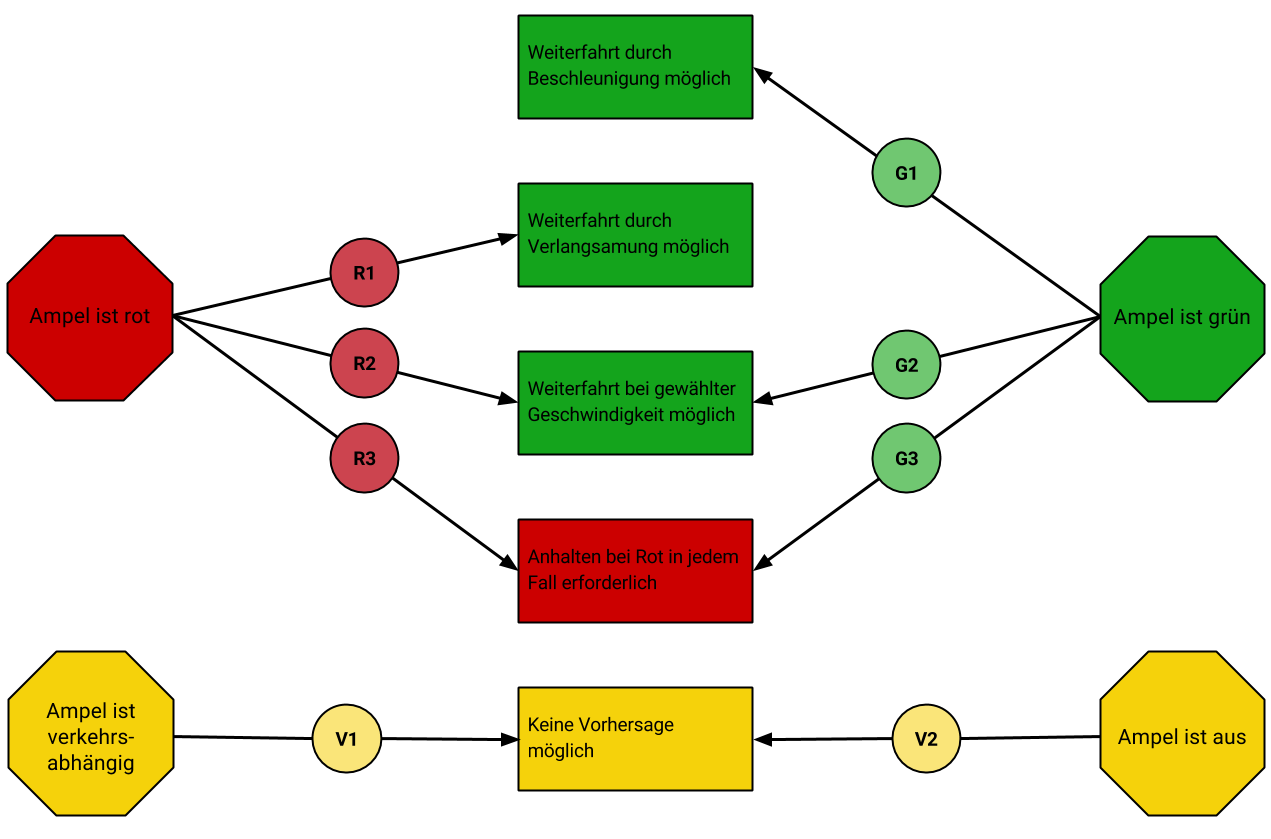
\includegraphics[width=1\textwidth]{Szenarien} 
    \grayRule
    \caption[Szenarien]{Szenarien im Ampelbereich}
    \label{fig:szenarien}
\end{figure} \vspace{17pt}
\begin{description}[leftmargin=0.7cm,style=nextline]
\clearpage
% ROT
\item[Szenario R1:] 
Die Fahrradfahrerin oder der Fahrradfahrer nähert sich einer aktuell roten Ampel. Die Anwendung zeigt den Countdown der Restrotzeit an und empfiehlt, langsamer zu fahren, um die Ampel ohne anzuhalten passieren zu können.  \\
\item[Szenario R2:] 
Die Fahrradfahrerin oder der Fahrradfahrer nähert sich einer aktuell roten Ampel. Die Anwendung zeigt an, dass eine Weiterfahrt bei gleichbleibender Geschwindigkeit gewährleistet ist. Es besteht kein Aktionsbedarf. \\
\item[Szenario R3:] 
Die Fahrradfahrerin oder der Fahrradfahrer nähert sich einer aktuell roten Ampel. Die Anwendung meldet, das Erreichen der Grünphase ist auch bei Geschwindigkeitsreduktion nicht möglich.\\%in jedem Fall
% GRÜN 
\item[Szenario G1:] 
Die Fahrradfahrerin oder der Fahrradfahrer nähert sich einer aktuell grünen Ampel. Die Anwendung zeigt den Countdown der Restgrünzeit an und empfiehlt schneller zu fahren, um die Ampel ohne anzuhalten passieren zu können.\\
\item[Szenario G2:] 
Die Fahrradfahrerin oder der Fahrradfahrer nähert sich einer aktuell grünen Ampel. Die Anwendung zeigt an, dass eine Weiterfahrt bei gleichbleibender Geschwindigkeit gewährleistet ist. Es besteht kein Aktionsbedarf.\\ 
\item[Szenario G3:] 
Die Fahrradfahrerin oder der Fahrradfahrer nähert sich einer aktuell grünen Ampel. Die Anwendung meldet, das Anhalten bei einer auf Rot umspringenden Ampel ist in jedem Fall erforderlich, da eine zu hohe Geschwindigkeit zum Erreichen der noch grünen Ampel erforderlich wäre.\\
% Verkehrsabgängig oder aus
\item[Szenario V1:] 
Die Fahrradfahrerin oder der Fahrradfahrer nähert sich einer ausgeschalteten Ampel. Es gibt weder Grün- noch Rotphasen. Das System zeigt an, dass die aktuelle Verkehrslage beurteilt und entsprechend gehandelt werden sollte.\\ 
\end{description}
\clearpage
\centerline{\grayRule}
Die obigen Szenarien gehen von einer gleichbleibenden Ampelschaltung aus. Insbesondere in Großstädten gibt es viele Faktoren, die die Ampelschaltung beeinflussen können, indem sie Grün anfordern. Deshalb kann hier Szanario V2 eintreten. Da keine Echtzeitdaten mit speziellen Technologien zur Verfügung stehen, sollte die Anwendung für die Berechnungen ausschließlich die intervallgesteuerten \glspl{LSA} berücksichtigen.\\
\centerline{\grayRule}
\begin{description}[leftmargin=0.7cm,style=nextline]
\item[Szenario V2:] 
Die Fahrradfahrerin oder der Fahrradfahrer nähert sich einer verkehrsabhängigen Ampel. Das bedeutet, die Schaltung ist unregelmäßig und die Wahrscheinlichkeit des Zutreffens der Vorhersage zu gering. Die Anwendung zeigt also an, dass es ihr nicht möglich ist, eine Vorhersage zu treffen.\\ 
\end{description} %\vspace{27pt}
% ERGEBNIS
\subsection*{Ergebnis}
Da die Szenarien \textit{R2} und \textit{G2}, die Szenarien \textit{R3} und \textit{G3} sowie die Szenazien\textit{V1} und \textit{V2} zusammengefasst werden können, ergeben sich aus den acht Szenarien im Ampelbereich die fünf nun aufgezählten Fälle.
\begin{itemize}
	\item Fall a: Anhalten bei Rot in jedem Fall erforderlich
	\item Fall b: Weiterfahrt mit gleichbleibender Geschwindigkeit möglich.\\ Kein Aktionsbedarf
	\item Fall c: Weiterfahrt bei Verlangsamung möglich
	\item Fall d: Weiterfahrt bei Beschleunigung möglich
	\item Fall e: Keine Vorhersage möglich
\end{itemize}
Im weiteren Verlauf dieser Arbeit wird unter anderem beschrieben wie diese Fälle in die Konzeption der zu entwickelnden Anwendung eingebunden werden.
